\section{Aproximações de tempo discreto}

\begin{frame}{Aproximações de tempo discreto}
\begin{block}{}
	O projeto de controladores de tempo discreto pode ser realizado de duas formas:
	
	\tikzmark{A}
	
	\vspace{-0.4cm}
	
	\begin{enumerate}
		\item Através de \textbf{aproximações discretas} do projeto realizado no domínio contínuo.
		\item \textbf{Diretamente} no domínio discreto por meio da transformada $ \mathcal{Z} $.
	\end{enumerate}
	
	\begin{tikzpicture}[overlay, remember picture]
	\draw[->] ($ (A) +(0.2,0) $) to [out=240,in=135] +(0.1,-1.6cm) node[name=EmB] {} node[right, name=Em] 
	{\textbf{Emulação:} dado $ H(s) $ deve-se obter $ H(z) $ por \textbf{aproximações}:};
	
	\draw ($ (EmB)+(0.2,-0.2) $) -- ++(0,-0.5) node[right=10pt] 
	{Integração numérica}
	-- ++(0,-1) node[right=10pt] {Mapeamento polo-zero};
	
	\draw[->] ($ (EmB)+(0.2,-0.7) $) -- +(8pt,0);
	\draw[->] ($ (EmB)+(0.2,-1.7) $) -- +(8pt,0);
	\end{tikzpicture}
	
	\vspace{2.2cm}
\end{block}
\end{frame}

\begin{frame}{Emulação}
\begin{block}{Introdução}
\begin{itemize}
    \item Trata-se de um método \textbf{indireto} para projetar um controlador discreto.
\end{itemize}
\textbf{Passos:}
\begin{enumerate}
    \item Planta contínua;
    \item Projeto de controlador contínuo;
    \item \textbf{Obtenção do controlador discreto que se aproxima do controlador contínuo (por meio de uma aproximação)};
    \item Análise de desempenho;
    \item Se necessário retornar ao segundo ou terceiro passo.
\end{enumerate}
\end{block}
\end{frame}

\begin{frame}{Integração numérica}
\begin{block}{Ideia}
\begin{itemize}
    \item A ideia da aproximação por integração numérica é representar uma função de transferência por uma equação diferencial. Após isto, derivar uma equação de diferenças aproximando a equação diferencial.
    \item Serão vistas \textbf{quatro aproximações para a integração numérica}:
    \begin{enumerate}
        \item Retangular para frente (Euler 1);
        \item Retangular para trás (Euler 2);
        \item Trapezoidal ou bilinear (Tustin);
        \item Bilinear com \textit{prewarping}.
    \end{enumerate}
\end{itemize}
\end{block}
\end{frame}

\begin{frame}{Integração numérica}
\begin{block}{Formulação matemática}
Considere a função de transferência de um \textbf{integrador}. O objetivo é obter um sistema discreto que represente aproximadamente essa função.
\[ G(s)=\dfrac{Y(s)}{U(s)}=\dfrac{1}{s}\Rightarrow \dot{y}(t)=u(t) \]
Integrando ambos os lados em um tempo de amostragem $ T $:
\[ \int_{(k-1)T}^{kT}\dot{y}(t)\dif t=\int_{(k-1)T}^{kT}u(t)\dif t\Rightarrow y(kT)-y[(k-1)T]=\int_{(k-1)T}^{kT}u(t)\dif t \]
\end{block}
\end{frame}


\begin{frame}{Retangular para frente (Euler 1)}
\centering

\vspace{-2.5cm}

\noindent
\scalebox{1}{\tikzset{every picture/.style={line width=0.75pt}} %set default line width to 0.75pt        

\begin{tikzpicture}[x=0.75pt,y=0.75pt,yscale=-1,xscale=1]
%uncomment if require: \path (0,300); %set diagram left start at 0, and has height of 300

\draw [pattern=south east lines, draw=white] (359.97,136.37) rectangle (407.73,242.57);

%Shape: Rectangle [id:dp8372137297740814] 
\draw  [][dash pattern={on 4.5pt off 4.5pt}] (359.97,136.37) -- (407.73,136.37) -- (407.73,242.57) -- (359.97,242.57) -- cycle ;

%Straight Lines [id:da9698438076731584] 
\draw [dash pattern={on 4.5pt off 4.5pt}]  (177.5,136.37) -- (359.97,136.37);

\draw[fill=black] (359.97,136.37) circle (1.2pt);

%Shape: Axis 2D [id:dp22952383480057992] 
\draw  (147,242.57) -- (445.67,242.57)(176.87,46.68) -- (176.87,264.33) (438.67,237.57) -- (445.67,242.57) -- (438.67,247.57) (171.87,53.68) -- (176.87,46.68) -- (181.87,53.68)  ;
%Curve Lines [id:da30754158713606405] 
\draw    (177.23,104.12) .. controls (296.48,-73.03) and (355.43,242.57) .. (437.05,136.46) ;

% Text Node
\draw (361.33,253.67) node   {$( k-1) T$};
% Text Node
\draw (410.33,253.67) node   {$kT$};
% Text Node
\draw (135,137) node   {$u[( k-1) T]$};


\end{tikzpicture}
}
\end{frame}


\begin{frame}{Retangular para frente (Euler 1)}
\begin{block}{Formulação matemática}
	\[ y(kT)-y[(k-1)T]=T u[(k-1)T] \]
	Aplicando a transformada $ \mathcal{Z} $ na equação acima, temos:
	\[ Y(z) - z^{-1}Y(z)=Tz^{-1}U(z) \]
	Portanto,
	\[ \dfrac{Y(z)}{U(z)}=\dfrac{Tz^{-1}}{1-z^{-1}}=\dfrac{T}{z-1} \]
	Lembre-se que $ \dfrac{Y(s)}{U(s)}=\dfrac{1}{s} $, logo
	\begin{gather*}
	\dfrac{1}{s}\approx\dfrac{T}{z-1}\Rightarrow\\
	\boxed{s=\dfrac{z-1}{T}} \text{ ou } \boxed{z=Ts+1}
	\end{gather*}
\end{block}
\end{frame}

\begin{frame}{Retangular para frente (Euler 1)}
\begin{block}{Estabilidade}
\begin{itemize}
\item Para analisar o limite de estabilidade, sabemos que $ s=j\omega $ mapeia-se em:
\end{itemize}
$$ z=Tj\omega+1 $$
\begin{itemize}
\item Para analisar a região de estabilidade, considere:
\end{itemize}
$$\Re(s) < 0 \implies \Re \left(\dfrac{z-1}{T}\right) < 0$$
\begin{itemize}
\vspace{-0.3cm}
\item[] Como $T > 0$, temos que:
\end{itemize}
$$\Re(z-1) < 0 \implies \Re(z) < 1$$
\end{block}
\end{frame}

\begin{frame}{Retangular para frente (Euler 1)}
\begin{block}{Estabilidade}
\begin{itemize}	
\item Portanto, sistemas estáveis no plano $ s $ podem se tornar \textbf{instáveis} quando mapeados para $ z $ (\textit{veja o exemplo a seguir -- pense em um valor de T que torne o equivalente discreto instável}).
\end{itemize}
\end{block}
\centering
\vspace{0.2cm}
\scalebox{0.9}{\begin{tikzpicture}[scale=1.5,>=latex, every node/.style={inner sep=2pt}]

	\draw[pattern=south east lines, draw=white, thin] (-1.5cm,-1.5cm) rectangle (1cm,1.5cm);

	% draw the unit circle
	\draw[line width=3pt, draw=white] (0cm,0cm) circle(1cm);
	\draw[thick] (0cm,0cm) circle(1cm);
	
    % draw the coordinates
    \draw[->, fill=white] (-1.5cm,0cm) -- (1.5cm,0cm) node[right=2pt,fill=white] {$\Re(z)$};
    \draw[->, fill=white] (0cm,-1.5cm) -- (0cm,1.5cm) node[above=2pt,fill=white] {$\Im(z)$};
    
    \draw[dashed, thick] (1,-1.5) -- (1,1.5);
    
    \draw (-1,0) node[inner sep=0.2pt,fill=white, below=1pt,xshift=-10pt] {$ -1 $};
    \draw (1,0) node[inner sep=0.2pt,below=1pt,xshift=5pt] {$ 1 $};
    \draw (0,1) node[inner sep=0.2pt,fill=white, right=2pt,yshift=5pt] {$ 1 $};
    \draw (0,-1) node[inner sep=0.2pt,fill=white, right=2pt,yshift=-7pt] {$ -1 $};
\end{tikzpicture}}
\end{frame}

\begin{frame}{Retangular para frente (Euler 1) - Exemplo \#01}
\begin{block}{Problema}
Discretize a função de transferência do controlador abaixo utilizando o método Euler 1, e considerando $T= \num{1}$ s.
	\[ C(s)=\dfrac{2}{s+2} \]
\end{block}
\end{frame}


\begin{frame}{Retangular para frente (Euler 1) - Exemplo \#01}
\begin{block}{Resolução}
	\[ C(z)=\dfrac{2}{\dfrac{z-1}{T}+2}=\dfrac{2T}{z-1+2T} \]
	\[ \dfrac{U(z)}{E(z)}=\dfrac{\num{2}}{z+\num{1}}\Rightarrow u[k+1]+u[k]=\num{2}e[k] \]
	Aplicando um atraso, temos:
	\[ u[k]=-u[k-1]+\num{2}e[k-1] \]
\end{block}
\end{frame}


\begin{frame}{Retangular para trás (Euler 2)}
\centering

\vspace{-2.5cm}

\scalebox{1}{\tikzset{every picture/.style={line width=0.75pt}} %set default line width to 0.75pt        

\begin{tikzpicture}[x=0.75pt,y=0.75pt,yscale=-1,xscale=1]
%uncomment if require: \path (0,300); %set diagram left start at 0, and has height of 300

\draw [pattern=south east lines, draw=white] (312.23,136.37) rectangle (359.97,242.57);

%Shape: Rectangle [id:dp8372137297740814] 
\draw  [dash pattern={on 4.5pt off 4.5pt}] (312.23,136.37) -- (359.97,136.37) -- (359.97,242.57) -- (312.23,242.57) -- cycle ;

\draw[fill=black] (359.97,136.37) circle (1.2pt);

%Shape: Axis 2D [id:dp22952383480057992] 
\draw  (147,242.57) -- (445.67,242.57)(176.87,46.68) -- (176.87,264.33) (438.67,237.57) -- (445.67,242.57) -- (438.67,247.57) (171.87,53.68) -- (176.87,46.68) -- (181.87,53.68)  ;
%Curve Lines [id:da30754158713606405] 
\draw    (177.23,104.12) .. controls (296.48,-73.03) and (355.43,242.57) .. (437.05,136.46) ;


%Straight Lines [id:da9698438076731584] 
\draw [dash pattern={on 4.5pt off 4.5pt}]  (177.5,136.37) -- (312.23,136.37) ;


% Text Node
\draw (315,253.67) node   {$( k-1) T$};
% Text Node
\draw (360.33,253.67) node   {$kT$};
% Text Node
\draw (150,137) node   {$u[ kT]$};


\end{tikzpicture}
}
\end{frame}


\begin{frame}{Retangular para trás (Euler 2)}
\begin{block}{Formulação matemática}
	\[ y(kT)-y[(k-1)T]=Tu(kT) \]
	Aplicando a transformada $ \mathcal{Z} $ na equação acima, temos:
	\[ Y(z)-z^{-1}Y(z)=TU(z) \]
	Portanto,
	\[ \dfrac{Y(z)}{U(z)}=\dfrac{T}{1-z^{-1}}=\dfrac{Tz}{z-1} \]
	Lembre-se que $ \dfrac{Y(s)}{U(s)}=\dfrac{1}{s} $, logo: \useshortskip
	\begin{gather*}
	\dfrac{1}{s}\approx\dfrac{Tz}{z-1}\Rightarrow\\
	\boxed{s=\dfrac{z-1}{Tz}}\text{ ou }\boxed{z=\dfrac{1}{1-Ts}}
	\end{gather*}
\end{block}
\end{frame}

\begin{frame}{Retangular para trás (Euler 2)}
\begin{block}{Estabilidade}
\begin{itemize}
\item Para analisar o limite de estabilidade, sabemos que $ s=j\omega $ mapeia-se em:
\end{itemize}
 \[ z=\dfrac{1}{1-Ts}+\dfrac{1}{2}-\dfrac{1}{2}=\dfrac{1}{2}+\dfrac{1}{2}\underbrace{\dfrac{Ts+1}{1-Ts}}_{\text{módulo}=1 \text{ p/ }s=j\omega} \implies |z-1/2|=1/2  \]
\begin{itemize}
\item Para analisar a região de estabilidade, considere:
\end{itemize}
$$\Re(s) < 0 \implies \Re \left(\dfrac{z-1}{Tz}\right) < 0$$
\begin{itemize}
\vspace{-0.3cm}
\item[] Como $T > 0$, temos que:
\end{itemize}
$$\Re \left(\dfrac{z-1}{z}\right) < 0 \implies \Re \left(\dfrac{a+jb-1}{a+jb}\right) < 0$$
\end{block}
\end{frame}

\begin{frame}{Retangular para trás (Euler 2)}
\begin{block}{Estabilidade}
\begin{itemize}
\item[] Multiplicando pelo conjugado, para separar a parte real da parte imaginária, temos:
\end{itemize}
$$\Re \left(\dfrac{(a-1)+jb}{a+jb} \cdot \dfrac{a-jb}{a-jb}\right) < 0 \implies \Re \left(\dfrac{a^2-a+bj+b^2}{a^2+b^2}\right) < 0$$
\begin{itemize}
\item[] Como o denominador é sempre maior que zero, temos que:
\end{itemize}
$$\Re (a^2-a+bj+b^2) < 0 \implies a^2-a+b^2 < 0$$
\begin{itemize}
\item[] Completando quadrados, podemos escrever:
\end{itemize}
$$(a-\num{0,5})^2+b^2 < \num{0,5}^2$$
\begin{itemize}
\vspace{-0.3cm}
\item[] o que representa uma circunferência de raio $\num{0,5}$ com centro deslocado em $\num{0,5}$ em $a$.
\end{itemize}
\end{block}
\end{frame}

\begin{frame}{Retangular para trás (Euler 2)}
\begin{block}{Estabilidade}
\begin{itemize}
	    \item Esta transformação mapeia sistemas estáveis em $ s $ em sistemas estáveis em $ z $. No entanto, \textbf{nem toda a região de estabilidade no plano $\bm{z}$ é usada}, restringindo o espaço do projeto (\textit{veja o exemplo a seguir -- existe algum valor de T que torne o equivalente discreto instável?})
\end{itemize}
\end{block}
\centering
\vspace{0.2cm}
\scalebox{0.8}{\begin{tikzpicture}[scale=1.5,>=latex,every node/.style={inner sep=2pt}]

	\draw[pattern=south east lines, draw=white, thin] (0.5cm,0) circle (0.5cm);
	
	\draw[dashed] (0.5,0) circle (0.5);
	
	% draw the unit circle
%	\draw[line width=3pt, draw=white] (0cm,0cm) circle(1cm);
	\draw (0cm,0cm) circle(1cm);
	
    % draw the coordinates
    \draw[->, fill=white] (-1.5cm,0cm) -- (1.5cm,0cm) node[right=2pt,fill=white] {$\Re(z)$};
    \draw[->, fill=white] (0cm,-1.5cm) -- (0cm,1.5cm) node[above=2pt,fill=white] {$\Im(z)$};
    
    \draw (-1,0) node[below,xshift=-7pt] {$ -1 $};
    \draw (1,0) node[below,xshift=5pt] {$ 1 $};
    \draw (0,1) node[right=2pt,yshift=5pt] {$ 1 $};
    \draw (0,-1) node[right=2pt,yshift=-5pt] {$ -1 $};
\end{tikzpicture}}
\end{frame}


\begin{frame}{Retangular para trás (Euler 2) - Exemplo \#01}
\begin{block}{Problema}
Discretize a função de transferência do controlador abaixo utilizando o método Euler 2, e considerando $T= \num{1}$ s.
	\[ C(s)=\dfrac{2}{s+2} \]
\end{block}
\end{frame}


\begin{frame}{Retangular para trás (Euler 2) - Exemplo \#01}
\begin{block}{Resolução}
	\[ C(z)=\dfrac{2}{\dfrac{z-1}{Tz}+2}=\dfrac{2Tz}{z(1+2T)-1} \]
	\[ \dfrac{U(z)}{E(z)}=\dfrac{\num{2}z}{\num{3}z-1}\Rightarrow \num{3}u[k+1]-u[k]=\num{2}e[k+1] \]
	Aplicando um atraso, e dividindo por $\num{3}$, temos:
	\[ u[k]=\dfrac{1}{3}u[k-1]+\dfrac{2}{3}e[k] \]
\end{block}
\end{frame}


\begin{frame}{Trapezoidal ou bilinear (Tustin)}
\centering

\vspace{-2.5cm}

\scalebox{1}{

\tikzset{every picture/.style={line width=0.75pt}} %set default line width to 0.75pt        

\begin{tikzpicture}[x=0.75pt,y=0.75pt,yscale=-1,xscale=1]
%uncomment if require: \path (0,300); %set diagram left start at 0, and has height of 300

%Straight Lines [id:da8305438567766523] 
\draw    (200.27,190.67) -- (365.77,190.67) ;
\draw [shift={(367.77,190.67)}, rotate = 180] [color={rgb, 255:red, 0; green, 0; blue, 0 }  ][line width=0.75]    (10.93,-3.29) .. controls (6.95,-1.4) and (3.31,-0.3) .. (0,0) .. controls (3.31,0.3) and (6.95,1.4) .. (10.93,3.29)   ;

%Shape: Circle [id:dp5343795865479193] 
\draw  [fill={rgb, 255:red, 255; green, 255; blue, 255 }  ,fill opacity=1 ] (347.47,190.58) .. controls (347.47,189.25) and (348.55,188.17) .. (349.88,188.17) .. controls (351.22,188.17) and (352.3,189.25) .. (352.3,190.58) .. controls (352.3,191.92) and (351.22,193) .. (349.88,193) .. controls (348.55,193) and (347.47,191.92) .. (347.47,190.58) -- cycle ;
%Shape: Circle [id:dp9958561748525927] 
\draw  [fill={rgb, 255:red, 255; green, 255; blue, 255 }  ,fill opacity=1 ] (328.07,190.68) .. controls (328.07,189.35) and (329.15,188.27) .. (330.48,188.27) .. controls (331.82,188.27) and (332.9,189.35) .. (332.9,190.68) .. controls (332.9,192.02) and (331.82,193.1) .. (330.48,193.1) .. controls (329.15,193.1) and (328.07,192.02) .. (328.07,190.68) -- cycle ;
%Straight Lines [id:da3574860753882376] 
\draw    (250.57,272.59) -- (250.57,191.28) ;


%Shape: Circle [id:dp04408180627185376] 
\draw  [fill={rgb, 255:red, 255; green, 255; blue, 255 }  ,fill opacity=1 ] (248.17,272.59) .. controls (248.17,273.92) and (249.24,275) .. (250.57,275) .. controls (251.9,275) and (252.98,273.92) .. (252.98,272.59) .. controls (252.98,271.26) and (251.9,270.18) .. (250.57,270.18) .. controls (249.24,270.18) and (248.17,271.26) .. (248.17,272.59) -- cycle ;
%Straight Lines [id:da7712579502140393] 
\draw    (270.5,251.85) -- (270.5,191.28) ;


%Shape: Circle [id:dp4215879501304003] 
\draw  [fill={rgb, 255:red, 255; green, 255; blue, 255 }  ,fill opacity=1 ] (268.1,251.85) .. controls (268.1,253.18) and (269.17,254.26) .. (270.5,254.26) .. controls (271.83,254.26) and (272.91,253.18) .. (272.91,251.85) .. controls (272.91,250.52) and (271.83,249.44) .. (270.5,249.44) .. controls (269.17,249.44) and (268.1,250.52) .. (268.1,251.85) -- cycle ;
%Straight Lines [id:da39800912811539835] 
\draw    (290.43,231.92) -- (290.43,191.28) ;


%Straight Lines [id:da15358320586768315] 
\draw    (310.86,210) -- (310.86,190.78) ;


%Shape: Circle [id:dp9326128099979845] 
\draw  [fill={rgb, 255:red, 255; green, 255; blue, 255 }  ,fill opacity=1 ] (288.02,231.92) .. controls (288.02,233.25) and (289.1,234.33) .. (290.43,234.33) .. controls (291.76,234.33) and (292.84,233.25) .. (292.84,231.92) .. controls (292.84,230.59) and (291.76,229.51) .. (290.43,229.51) .. controls (289.1,229.51) and (288.02,230.59) .. (288.02,231.92) -- cycle ;
%Shape: Circle [id:dp7866868035269907] 
\draw  [fill={rgb, 255:red, 255; green, 255; blue, 255 }  ,fill opacity=1 ] (308.45,212.41) .. controls (308.45,213.74) and (309.53,214.81) .. (310.86,214.81) .. controls (312.19,214.81) and (313.27,213.74) .. (313.27,212.41) .. controls (313.27,211.08) and (312.19,210) .. (310.86,210) .. controls (309.53,210) and (308.45,211.08) .. (308.45,212.41) -- cycle ;

% Text Node
\draw (224,203) node   {$\dotsc $};
% Text Node
\draw (371.5,197) node   {$n$};
% Text Node
\draw (310,180) node   {$-1$};
% Text Node
\draw (287,180) node   {$-2$};
% Text Node
\draw (265,180) node   {$-3$};
% Text Node
\draw (246,180) node   {$-4$};


\end{tikzpicture}
}
\end{frame}


\begin{frame}{Trapezoidal ou bilinear (Tustin)}
\begin{block}{Formulação matemática}
	\[ y(kT)-y[(k-1)T]=\dfrac{T}{2}\left( u(kT)+u[(k-1)T] \right) \]
	Aplicando a transformada $ \mathcal{Z} $ na equação acima, temos: \useshortskip
	\[ Y(z)-z^{-1}Y(Z)=\dfrac{T}{2}\left( U(z)+z^{-1}U(z) \right) \]
	Portanto, \useshortskip
	\[ \dfrac{Y(z)}{U(z)}=\dfrac{T}{2}\dfrac{(1+z^{-1})}{(1-z^{-1})}=\dfrac{T}{2}\dfrac{(z+1)}{(z-1)} \]
	Lembre-se que $ \dfrac{Y(s)}{U(s)}=\dfrac{1}{s} $, logo: \useshortskip
	\begin{gather*}
	\dfrac{1}{s}\approx\dfrac{T}{2}\dfrac{(z+1)}{(z-1)}\Rightarrow\\
	\boxed{s=\dfrac{2}{T}\dfrac{(z-1)}{(z+1)}}\text{ ou }\boxed{z=\dfrac{1+Ts/2}{1-Ts/2}}
	\end{gather*}
\end{block}
\end{frame}

\begin{frame}{Trapezoidal ou bilinear (Tustin)}
\begin{block}{Estabilidade}
\begin{itemize}
\item Para analisar o limite de estabilidade, sabemos que $ s=j\omega $ mapeia-se em:
\end{itemize}
	\[ z=\underbrace{\dfrac{1+\dfrac{Ts}{2}}{1-\dfrac{Ts}{2}}}_{\text{módulo}=1 \text{ p/ }s=j\omega} \]
\begin{itemize}
\item Para analisar a região de estabilidade, considere:
\end{itemize}
$$\Re(s) < 0 \implies \Re \left(\dfrac{2}{T}\dfrac{(z-1)}{(z+1)}\right) < 0$$
\begin{itemize}
\vspace{-0.3cm}
\item[] Como $2/T > 0$, temos que:
\end{itemize}
$$\Re \left(\dfrac{z-1}{z+1}\right) < 0 \implies \Re \left(\dfrac{a+jb-1}{a+jb+1}\right) < 0$$
\end{block}
\end{frame}

\begin{frame}{Trapezoidal ou bilinear (Tustin)}
\begin{block}{Estabilidade}
\begin{itemize}
\item[] Multiplicando pelo conjugado, para separar a parte real da parte imaginária, temos:
\end{itemize}
$$\Re \left(\dfrac{(a-1)+jb}{(a+1)+jb} \cdot \dfrac{a+1 -jb}{a+1 -jb}\right) < 0 \implies \Re \left(\dfrac{a^2-1+2bj+b^2}{(a+1)^2+b^2}\right) < 0$$
\begin{itemize}
\item[] Como o denominador é sempre maior que zero, temos que:
\end{itemize}
$$\Re (a^2-1+2bj+b^2) < 0 \implies a^2-1+b^2 < 0$$
\begin{itemize}
\item[] Com isso,
\end{itemize}
$$a^2+b^2 < 1^2$$
\begin{itemize}
\vspace{-0.3cm}
\item[] o que representa uma circunferência de raio unitário centrada na origem.
\end{itemize}
\end{block}
\end{frame}


\begin{frame}{Trapezoidal ou bilinear (Tustin)}
\begin{block}{Estabilidade}
\begin{itemize}
    \item Há o mapeamento de \textbf{todo semiplano esquerdo de $ \bm{s} $ no interior do círculo unitário de $ \bm{z} $} (\textit{veja o exemplo a seguir -- existe algum valor de T que torne o equivalente discreto instável?})
\end{itemize}
\end{block}

\centering

\scalebox{0.9}{\deftkzbds

\begin{tikzpicture}[auto, node distance=1cm,>=Latex]
	% We start by placing the blocks
	\node [input] (input) {};
	\node [right=1cm, name=mid1, node distance=1pt, inner sep=1pt, fill=black, circle, draw] at (input) {};
	\node [right=1.3cm, name=mid] at (mid1) {};
	\node [block, above=0.5cm] at (mid) (h1) {$ h_1[n] $};
	\node [block, below=0.5cm] at (mid) (h2) {$ h_2[n] $};
	\node [sum, right=1cm, name=sum] at (mid) {$ + $};
	\node [output, right =of sum] (output) {};
	\node [above] at (input) {$ z^{n} $};
	\node [above] at (output) {$ y[n] $};
	
	\draw [->] (input) -| (mid1) |- (h1);
	\draw [->] (mid1) |- (h2);
	\draw [->] (h1) -| node[midway,right] {$ y_1[n] $} (sum);
	\draw [->] (h2) -| node[midway,right] {$ y_2[n] $} (sum);
	\draw [->] (sum) -- (output);
	
	\node[right=0.5cm, name=eq] at (output) {\Large $ \equiv $};
	
	\node [input, right=0.5cm] at (eq) (in2) {};
	\node [block, right=of in2] (computer) {$ x[n] $};
	\node [output, right =of computer] (out2) {};
	\node [above] at (in2) {$ z^{n} $};
	\node [above] at (out2) {$ y[n] $};
	
	\draw [->] (in2) -- (computer);
	\draw [->] (computer) -- (out2);
\end{tikzpicture}}
\end{frame}

\begin{frame}{Trapezoidal ou bilinear (Tustin) - Exemplo \#01}
\begin{block}{Problema}
Discretize a função de transferência do controlador abaixo utilizando o método de Tustin, e considerando $T= \num{1}$ s.
	\[ C(s)=\dfrac{2}{s+2} \]
\end{block}
\end{frame}


\begin{frame}{Trapezoidal ou bilinear (Tustin) - Exemplo \#01}
\begin{block}{Resolução}
	\[ C(z)=\dfrac{2}{\dfrac{2}{T}\dfrac{(z-1)}{(z+1)}+2}=\dfrac{2T(z+1)}{2(z-1)+2T(z+1)} \]
	\[ \dfrac{U(z)}{E(z)}=\dfrac{\num{0,5}z+\num{0,5}}{z}\Rightarrow u[k+1]=\num{0,5}e[k+1]+\num{0,5}e[k] \]
	Aplicando um atraso, temos:
	\[ u[k]=\num{0,5}e[k]+\num{0,5}e[k-1] \]
\end{block}
\end{frame}

\cprotect\frame{
\frametitle{\MATLAB}
\begin{block}{}
\begin{verbatim}
>>c2d(sys,T,'tustin') 
\end{verbatim}
converte um sistema dinâmico de tempo contínuo \textbf{sys} em tempo discreto com um tempo de amostragem $\bm{T}$ utilizando o método \textbf{tustin}. \\
\vspace{0.2cm}
\textbf{Exemplo}: discretização do exemplo \#01
\end{block}
\centerline{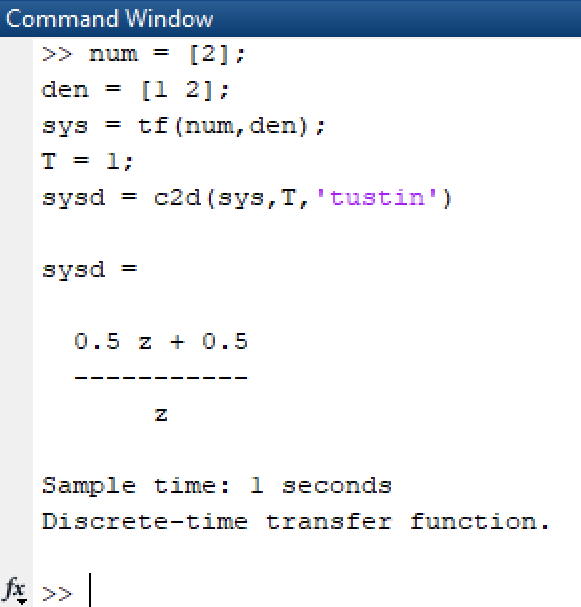
\includegraphics[width=0.4\linewidth]{Figuras/Ch08/fig1.PNG}}
}

\begin{frame}{Bilinear com \textit{prewarping}}
\begin{block}{Origem do \textit{warping}}
\begin{itemize}
    \item O \textit{warping} é uma distorção não linear na frequência quando há a transição entre o plano $s$ e o plano $z$, dependendo da frequência utilizada.
    \item No caso de sistemas como \textbf{filtros} (onde a preservação do comportamento da frequência é extremamente importante) esta transformação torna-se ineficaz.
    \item As características da resposta em frequência do filtro analógico aparecem no filtro digital. No entanto, a escala de frequência com que a resposta ocorre sofrerá uma \textbf{compressão de um intervalo infinito para um intervalo finito}.
    \item Todo o eixo $j\omega$ é \textbf{comprimido} no círculo unitário de comprimento $2\pi$, causando uma \textbf{distorção de frequência}.
\end{itemize}
\end{block}
\end{frame}

\begin{frame}{Bilinear com \textit{prewarping}}
\begin{block}{Formulação matemática}
Considere que um ponto no plano $s$ é dado por $\sigma + j\omega_a$. Como a parte real não é afetada pela frequência, podemos escrever:
$$s = j\omega_a$$
De semelhante modo, um ponto no plano $z$ (também desconsiderando a parte que não é afetada pela frequência) é dado por:
$$z = \text{e}^{j\omega_dT}$$
Por Tustin sabemos que:
$$s=\dfrac{2}{T}\dfrac{(z-1)}{(z+1)} \implies
j\omega_a = \dfrac{2}{T}\dfrac{(\text{e}^{j\omega_dT}-1)}{(\text{e}^{j\omega_dT}+1)}$$
\end{block}
\end{frame}

\begin{frame}{Bilinear com \textit{prewarping}}
\begin{block}{Formulação matemática}
\begin{align*}
    j\omega_a &= \dfrac{2}{T}\dfrac{(\text{e}^{j\omega_dT}-1)}{(\text{e}^{j\omega_dT}+1)} \\ \\
    j\omega_a &= \dfrac{2}{T}\dfrac{\text{e}^{j\omega_dT/2}(\text{e}^{j\omega_dT/2}-\text{e}^{-j\omega_dT/2})}{\text{e}^{j\omega_dT/2}(\text{e}^{j\omega_dT/2}+\text{e}^{-j\omega_dT/2})} \\ \\
    j\omega_a &= j\dfrac{2}{T}\dfrac{\dfrac{\text{e}^{j\omega_dT/2}-\text{e}^{-j\omega_dT/2}}{2j}}{\dfrac{\text{e}^{j\omega_dT/2}+\text{e}^{-j\omega_dT/2}}{2}} = j\dfrac{2}{T}\dfrac{\text{sen}(\omega_dT/2)}{\text{cos}(\omega_dT/2)} \implies
\end{align*}
$$\boxed{\omega_a = \dfrac{2}{T}\text{tan}(\omega_dT/2)} \text{ ou } \boxed{\omega_d = \dfrac{2}{T}\text{tan}^{-1}(\omega_aT/2)}$$
\end{block}
\end{frame}

\begin{frame}{Bilinear com \textit{prewarping}}
\begin{block}{\textit{Prewarping}}
\begin{itemize}
    \item A correção \textit{prewarping} tem por objetivo antecipar a distorção da frequência no plano $s$, para amenizar a distorção quando a transformação for realizada. 
    \item A correção da distorção não é feita para todos os polos, amenizando apenas a distorção no \textbf{polo desejado}. Assim, a distorção ainda existe quando comparado com outro polo.
    \item Para aplicar a correção de \textit{prewarping}, é necessário utilizar a equação abaixo para calcular novos polos e zeros a partir dos originais. Feito isto, a transformação bilinear só será realizada após obter a nova função de transferência com polos e zeros corrigidos.
\end{itemize}
$$\boxed{\Bar{a} = \dfrac{2}{T} \text{tan} \left(\dfrac{aT}{2}\right)}$$
\end{block}
\end{frame}

\begin{frame}{Bilinear com \textit{prewarping}}
\begin{block}{Antes do \textit{prewarping}}
\begin{itemize}
    \item É possível observar que a distorção ocorre, porém mais amenizada em frequências menores.
\end{itemize}
\end{block}
\centerline{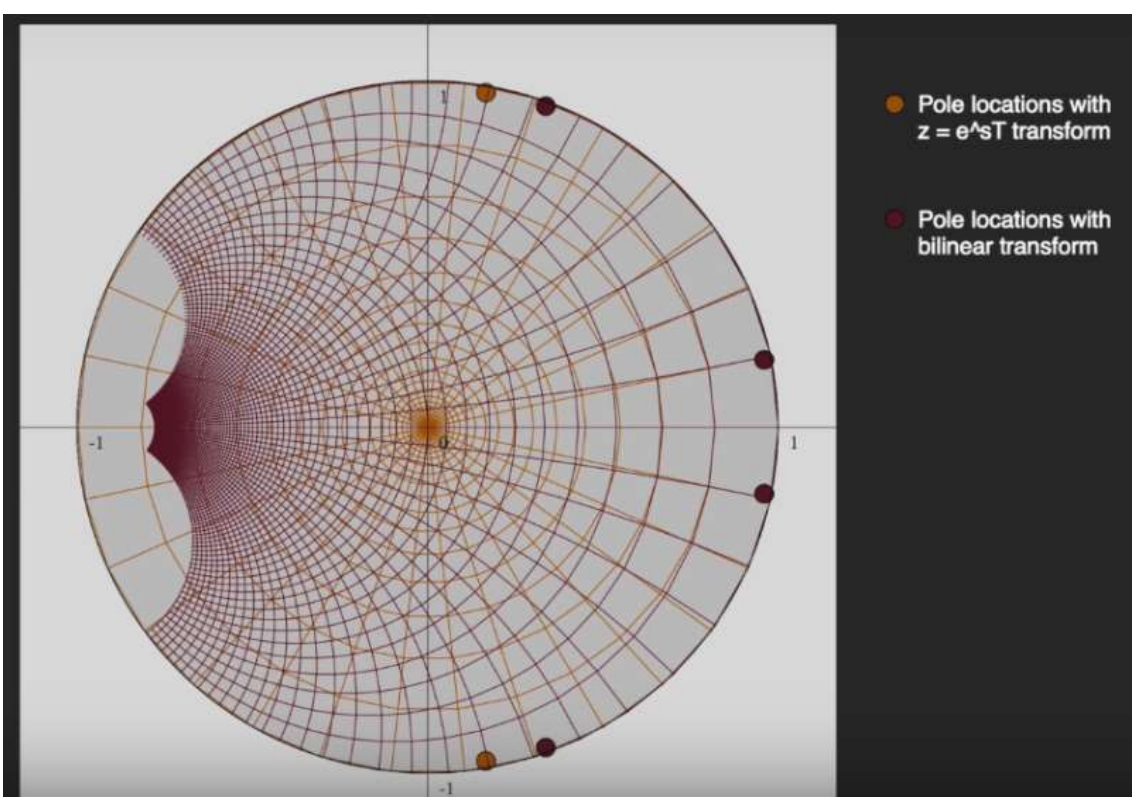
\includegraphics[width=0.65\linewidth]{Figuras/Ch08/fig2.PNG}}
\end{frame}

\begin{frame}{Bilinear com \textit{prewarping}}
\begin{block}{Depois do \textit{prewarping}}
\begin{itemize}
    \item Após a correção de \textit{prewarping}, pode ser observado que os polos de maior frequência no plano $z$ estão sem distorção. Entretanto, os polos de menor frequência sofreram certa distorção. 
\end{itemize}
\end{block}
\centerline{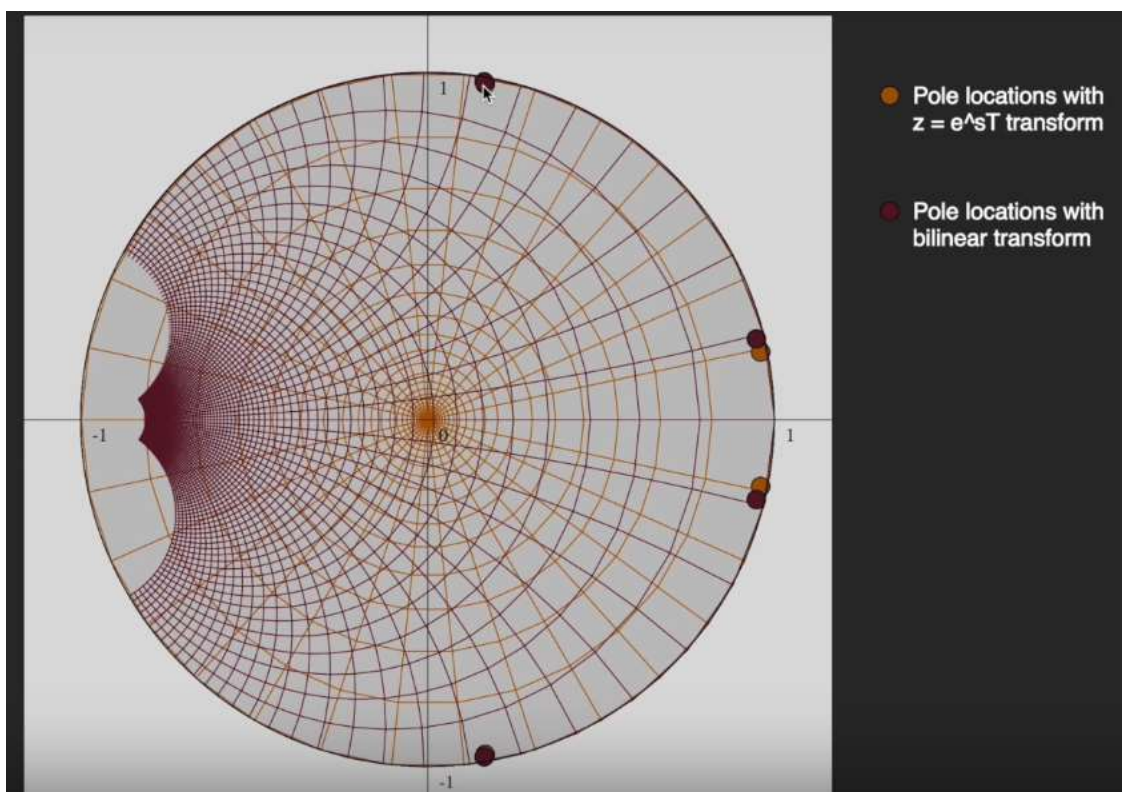
\includegraphics[width=0.65\linewidth]{Figuras/Ch08/fig3.PNG}}
\end{frame}

\begin{frame}{Bilinear com \textit{prewarping} - Exemplo \#01}
\begin{block}{Problema}
Discretize a função de transferência do controlador abaixo utilizando o método bilinear com \textit{prewarping} na frequência de corte do filtro, e considerando $T= \num{1}$ s.
	\[ C(s)=\dfrac{2}{s+2} \]
\end{block}
\end{frame}

\begin{frame}{Bilinear com \textit{prewarping} - Exemplo \#01}
\begin{block}{Resolução}
    \[ C(s)=\dfrac{\dfrac{2}{T} \text{tan} \left(\dfrac{aT}{2}\right)}{s+\dfrac{2}{T} \text{tan} \left(\dfrac{aT}{2}\right)} = \dfrac{2 \ \text{tan}(1)}{s+2 \ \text{tan}(1)} \]
	\[ C(z)=\dfrac{2 \ \text{tan}(1)}{\dfrac{2}{T}\dfrac{(z-1)}{(z+1)}+2 \ \text{tan}(1)}=\dfrac{2T(z+1) \ \text{tan}(1)}{2(z-1)+2T(z+1) \ \text{tan}(1)} \]
	\[ \dfrac{U(z)}{E(z)}=\dfrac{\num{0,609}z+\num{0,609}}{z + \num{0,218}}\Rightarrow u[k+1] + \num{0,218} u[k] =\num{0,609}e[k+1]+\num{0,609}e[k] \]
	Aplicando um atraso, temos:
	\[ u[k]=-\num{0,218}u[k-1]+\num{0,609}e[k]+\num{0,609}e[k-1] \]
\end{block}
\end{frame}

\cprotect\frame{
\frametitle{\MATLAB}
\begin{block}{}
\begin{verbatim}
>>c2d(sys,T,c2dOptions('Method','tustin','PrewarpFrequency',2))
\end{verbatim}
converte um sistema dinâmico de tempo contínuo \textbf{sys} em tempo discreto com um tempo de amostragem $\bm{T}$ utilizando o método \textbf{tustin} com \textbf{\textit{prewaping}} na frequência $\bm{w}$. \\
\vspace{0.2cm}
\textbf{Exemplo}: discretização do exemplo \#01
\end{block}
\centerline{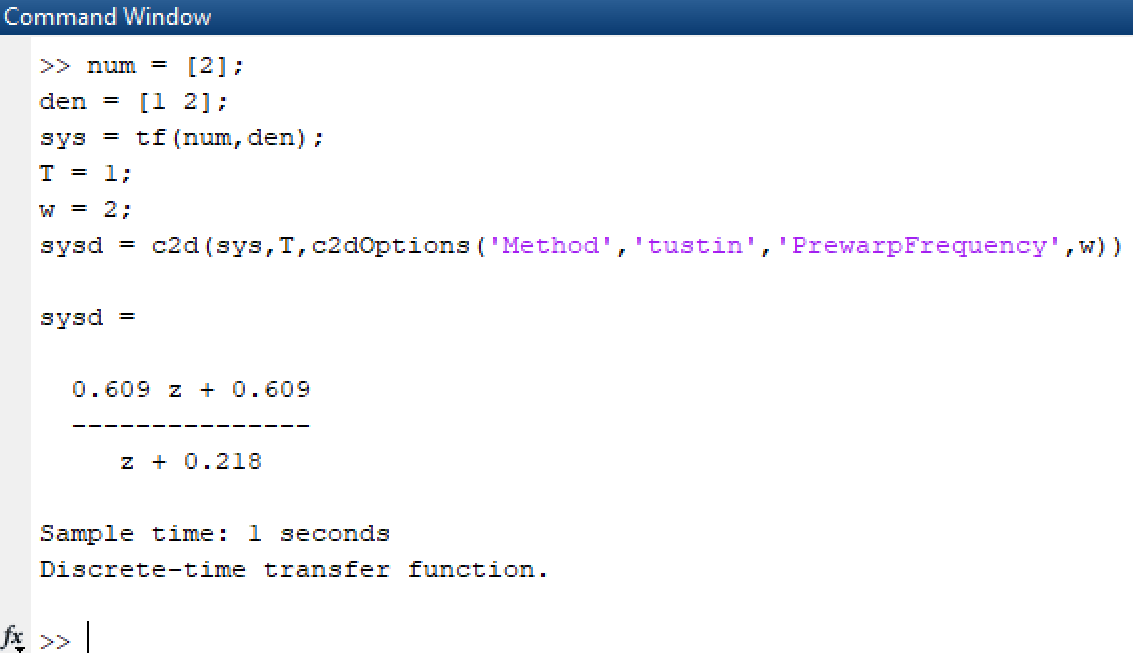
\includegraphics[width=0.6\linewidth]{Figuras/Ch08/fig4.PNG}}
}

\begin{frame}{\MATLAB}
\begin{block}{Antes do \textit{prewarping}}
\begin{itemize}
    \item Frequência de corte $\omega = 2$ rad/s.
\end{itemize}
\end{block}
\centerline{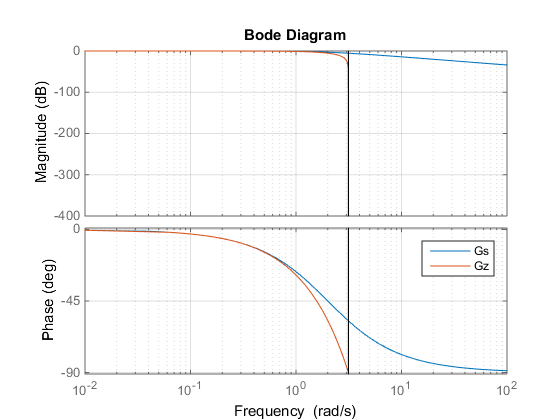
\includegraphics[width=0.7\linewidth]{Figuras/Ch08/fig5.png}}
\end{frame}

\begin{frame}{\MATLAB}
\begin{block}{Antes do \textit{prewarping}}
\begin{itemize}
    \item Frequência de corte $\omega = 2$ rad/s.
\end{itemize}
\end{block}
\centerline{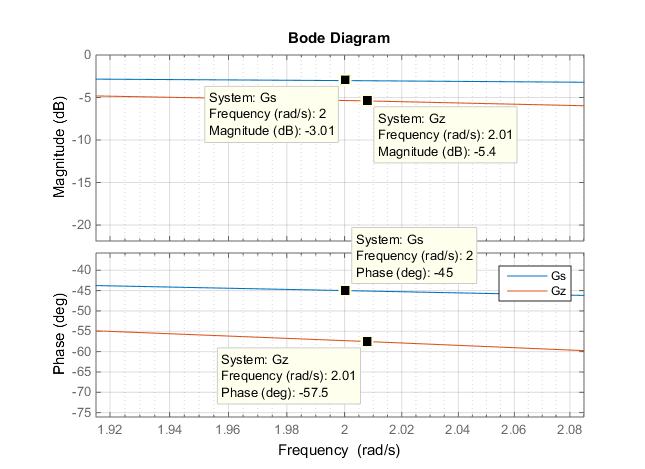
\includegraphics[width=0.7\linewidth]{Figuras/Ch08/fig6.png}}
\end{frame}

\begin{frame}{\MATLAB}
\begin{block}{Depois do \textit{prewarping}}
\begin{itemize}
    \item Frequência de corte $\omega = 2$ rad/s.
\end{itemize}
\end{block}
\centerline{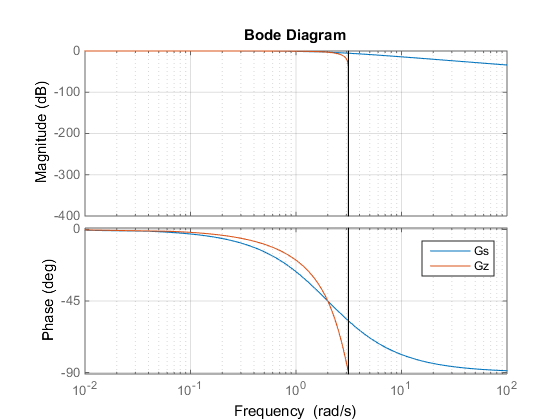
\includegraphics[width=0.7\linewidth]{Figuras/Ch08/fig7.png}}
\end{frame}

\begin{frame}{\MATLAB}
\begin{block}{Depois do \textit{prewarping}}
\begin{itemize}
    \item Frequência de corte $\omega = 2$ rad/s.
\end{itemize}
\end{block}
\centerline{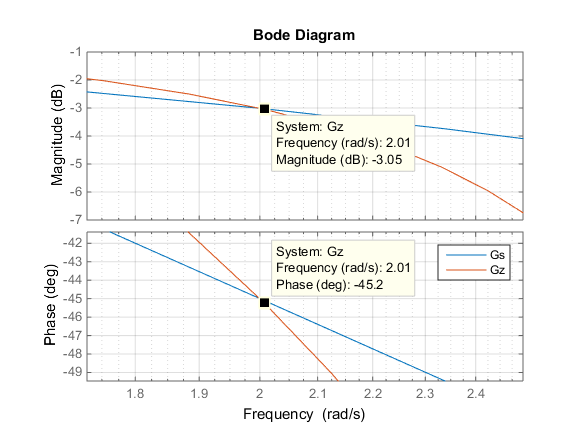
\includegraphics[width=0.7\linewidth]{Figuras/Ch08/fig8.png}}
\end{frame}

\begin{frame}{Bilinear com \textit{prewarping}}
\begin{block}{Observação}
\begin{itemize}
    \item E se a função de transferência contínua possuir mais de um polo?
\end{itemize}
$$G(z)=G(s)\Big|_{s=\dfrac{a(z-1)}{\left[\text{tan}\left(\dfrac{aT}{2}\right)\right](z+1)}}$$
\begin{itemize}
    \item[] onde $a$ é a frequência onde deseja-se que os ganhos dos sistemas contínuos e discretos sejam iguais.
\end{itemize}
\end{block}
\end{frame}

\begin{frame}{Mapeamento polo-zero}
\begin{block}{Ideia}
Obtém-se o equivalente discreto através da relação $ \bm{z=\text{\textbf{e}}^{sT}} $.
\begin{itemize}
    \item Se tomarmos a transformada $\mathcal{Z}$ de amostras de um sinal contínuo $e(t)$, então os \textbf{polos} da função de transferência discreta $E(z)$ estão relacionados aos polos de $E(s)$ de acordo com $z=\text{\textbf{e}}^{sT}$. No entanto, precisaríamos passar pelo mesmo processo de transformada $\mathcal{Z}$ para localizar os zeros de $E(z)$.
    \item A ideia da técnica do mapeamento polo-zero é que a relação $z=\text{\textbf{e}}^{sT}$ também pode ser razoavelmente aplicada para os \textbf{zeros} da função de transferência discreta.
\end{itemize}
\end{block}
\end{frame}

\begin{frame}{Mapeamento polo-zero}
	\begin{block}{Passos}
		\begin{enumerate}
			\item Inicialmente deve-se \textbf{fatorar} $ H(s) $ na forma de seus polos e zeros:\[ H(s)=K\cdot\dfrac{(s-z_1)(s-z_2)\cdots(s-z_m)}{(s-p_1)(s-p_2)\cdots(s-p_n)} \]
			
			\item Se $ H(s) $ possui um polo em $ s=-a $, $ H(z) $ possui um polo em $ z=\text{e}^{-aT} $.
			
			\item Se $ H(s) $ possui um polo em $ s=-a+jb $, $ H(z) $ possui um polo em $ z=r\text{e}^{j\theta} $, onde $ r=\text{e}^{-aT} $  e $ \theta=bT $.
			
			\item Todos os zeros finitos são mapeados do mesmo jeito que os polos (passos 2 e 3).
		\end{enumerate}
	\end{block}
\end{frame}


\begin{frame}{Mapeamento polo-zero}
	\begin{block}{Passos}
		\begin{enumerate}
			\setcounter{enumi}{4}
			\item Os zeros de $ H(s) $ em $ s\to\infty\,(m<n) $ são mapeados em $ \bm{z=-1} $. Acrescenta-se $\bm{n-m-1}$ fatores de $(z+1)$ ao numerador de $H(z)$. 
			\begin{itemize}
			    \item Esta regra permite que o computador tenha tempo para calcular a saída discreta (\textit{delay} de um tempo de amostragem).
			    \item O ponto $z = -1$ representa, de maneira real, a maior frequência possível na função de transferência discreta; portanto, é apropriado que se $H(s)$ for zero na maior frequência contínua, $|H(z)|$ deve ser zero em $z=-1$, a frequência mais alta que pode ser processada pelo filtro digital.
			\end{itemize}
			
			
			\item Ajusta-se o ganho de $ G(z) $, isto é, o \textbf{ganho} deve ser ajustado para que em baixa frequência essas funções possuam módulos iguais.
			
			\[ G(s)\Big|_{s=0}=G(z)\Big|_{z=1} \]
		\end{enumerate}
	\end{block}
\end{frame}

\begin{frame}{Mapeamento polo-zero - Exemplo \#01}
\begin{block}{Problema}
Discretize a função de transferência do controlador abaixo utilizando o mapeamento polo-zero, e considerando $T= \num{1}$ s.
	\[ C(s)=\dfrac{2}{s+2} \]
\end{block}
\end{frame}

\begin{frame}{Mapeamento polo-zero - Exemplo \#01}
\begin{block}{Resolução}
	\begin{enumerate}
		\item N/A.
		
		\item $ C(s) $ possui polo em $ s=-2 $, logo $ C(z) $ possui polo em $ z=\text{e}^{-2T}=\num{0,1353} $.
		
		\item N/A.
		
		\item N/A.
		
		\item N/A.
		
		\[ C(z)=\dfrac{K}{z-\num{0,1353}} \]
		
		\item
		\[
		C(s)\Big|_{s=0}=C(z)\Big|_{z=1}\Rightarrow 1=\dfrac{K}{\num{0,8647}}\Rightarrow K=\num{0,8647} \]
	\end{enumerate}
\end{block}
\end{frame}

\begin{frame}{Mapeamento polo-zero - Exemplo \#01}
\begin{block}{Resolução}
    \[ \dfrac{U(z)}{E(z)}=\dfrac{\num{0,8647}}{z-\num{0,1353}}\Rightarrow u[k+1] - \num{0,1353} u[k]=\num{0,8647}e[k] \]
	Aplicando um atraso, temos:
	\[ u[k]=\num{0,1353}u[k-1]+\num{0,8647}e[k-1] \]
\end{block}
\end{frame}

\cprotect\frame{
\frametitle{\MATLAB}
\begin{block}{}
\begin{verbatim}
>>c2d(sys,T,'matched') 
\end{verbatim}
converte um sistema dinâmico de tempo contínuo \textbf{sys} em tempo discreto com um tempo de amostragem $\bm{T}$ utilizando o método \textbf{matched} (\textit{mapeamento polo-zero}). \\
\vspace{0.2cm}
\textbf{Exemplo}: discretização do exemplo \#01
\end{block}
\centerline{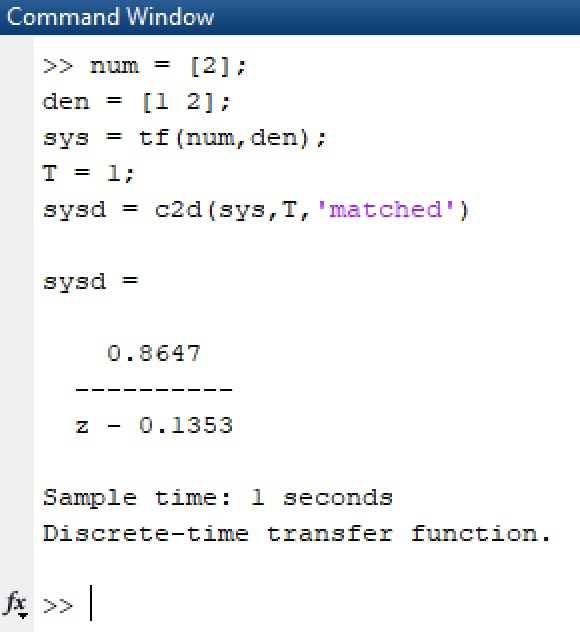
\includegraphics[width=0.35\linewidth]{Figuras/Ch08/fig9.PNG}}
}

\frame{
\frametitle{Exercícios}
\begin{block}{}
01. Mostre a equivalência dos métodos de discretização quando $T \to 0$.

\vspace{1cm}

02. A função de transferência abaixo é um compensador de avanço de fase projetado para adicionar aproximadamente \SI{60}{\degree} em $\omega_1 = 3$ rad:
$$H(s) = \dfrac{s+1}{0,1s+1}$$
Para cada um dos métodos de aproximação, calcule e desenhe no plano $\mathcal{Z}$ a localização dos polos e zeros da função de transferência discreta. Utilize $T = 0,25$ s.
\end{block}
}

\frame{
\frametitle{Exercícios}
\begin{block}{}
03. Encontre o equivalente discreto da função de transferência abaixo utilizando o método de Tustin. Faça também uma compensação de distorção em frequência para $a = 2$ rad/s e $T = 1$ s. Confira a sua resposta no \MATLAB por meio do diagrama de Bode.
$$G(s) = \dfrac{5}{s^2+3s+2}$$

\vspace{1cm}

04. Considerando a função de transferência genérica de primeira ordem
$$G(s) = \dfrac{a}{s+a}$$
Mostre que na frequência de canto, $|G(s)| = |G(z)| = \dfrac{1}{\sqrt{2}} = -\num{3,01}$ dB. 
\end{block}
}

\frame{
\frametitle{Referências e exercícios complementares}
\begin{itemize}
\item AGUIRRE, Luis A. Controle de Sistemas Amostrados, 1 ed. [s.n.], 2019.
\end{itemize}
\centering{\alert{Página 125 - \textbf{Capítulo 4}}} \\
\vspace{0.4cm}
\begin{itemize}
\item FRANKLIN, Gene F.; POWELL, J. David; WOLKMAN, Michael L. Digital Control of Dynamic Systems, 3 ed. Addison-Wesley, 1998.
\end{itemize}
\centering{\alert{Página 209 - \textbf{Capítulo 6}}} \\
}